\documentclass{article}
\usepackage[utf8]{inputenc}

\usepackage[OT2]{fontenc}
\usepackage[serbianc, serbian]{babel}
\usepackage{graphicx}
\usepackage{hyperref}

\usepackage{subfiles}
\usepackage{array}
\usepackage{float}

\title{\textbf{Informacioni sistem za menad2ment transporta shec1era na podruchju Republike Srbije}}
\author{Milica Gajic1, Marija Eric1, Milosh Kutleshic1\\
$milica@gmail.com$, $marija.eric@matf.bg.ac.rs$, $gamisn97@gmail.com$}

\begin{document}

\maketitle
\newpage


\renewcommand*\contentsname{Sadrz1aj}
\tableofcontents
\newpage

\section{Uvod}
\subfile{uvod}

\section{Sluchajevi upotrebe}
Prvi korak u razvoju je analiza sistema. Osnovni procesi c1e biti opisani kroz sluchajeve upotrebe. 
Na slici \ref{sistem} se mogu pronac1i svi prepoznati sluchajevi upotrebe, koji c1e u nastavku poglavlja biti detaljno opisani.
\begin{figure}[H]
    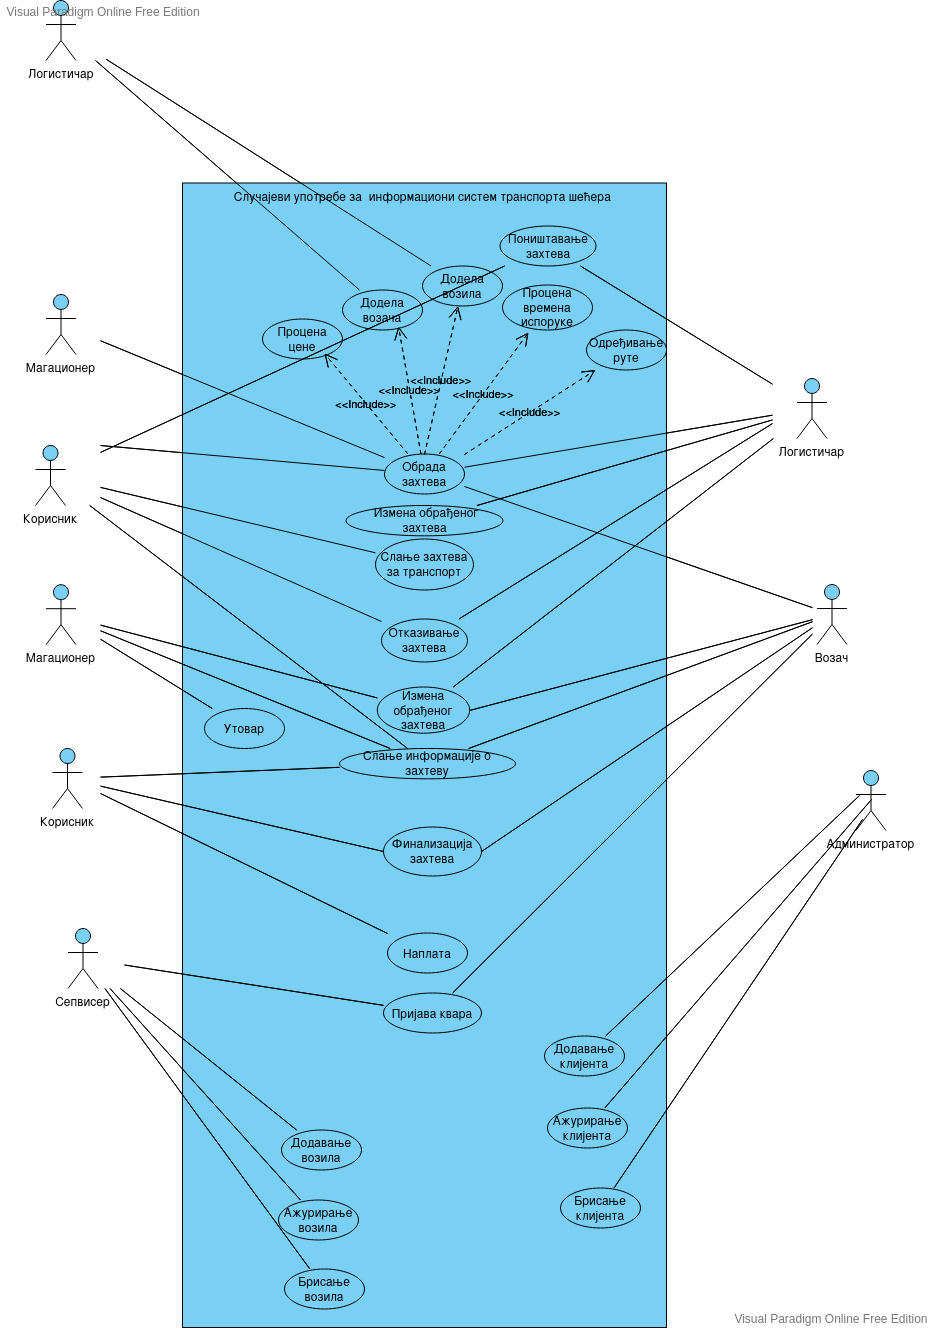
\includegraphics[scale = 0.4]{Slike/UML/SlucajeviUpotrebeSistema.jpg}
    \centering
    \caption{Sluchajevi upotrebe sistema za organizaciju transporta shec1era}
    \label{sistem}
\end{figure}  
Radi preglednosti sluchajevi upotrebe su grupisani u naredne kategorije:

\begin{itemize}
    \item Administrativni poslovi
    \item Logistika i transport
    \item Odrzhavanje vozila
\end{itemize}

\subsection{Administrativni poslovi}

\subfile{SlucajeviUpotrebe/SUadministrativniPoslovi}

\subsection{Logistika i transport}
U okviru logistike i transporta se nalaze svi sluchajevi upotrebe koji su vezani za proces planiranja transporta, od slanja zahteva, preko planiranja rute, pa do realizacije transporta do lokacije.
     
\subsubsection{Sluchaj upotrebe: Slanje zahteva za transport}
\subfile{SlucajeviUpotrebe/SUslanjeZahteva}

\subsubsection{Sluchaj upotrebe: Obrada zahteva za transport}
\subfile{SlucajeviUpotrebe/SUobradaZahteva}

\subsubsection{Sluchaj upotrebe: Izmena zahteva za transport}
\subfile{SlucajeviUpotrebe/SUizmenaZahteva.tex}

\subsubsection{Sluchaj upotrebe: Ponishtavanje zahteva za transport}
\subfile{SlucajeviUpotrebe/SUponistavanjeZahteva.tex}

\subsubsection{Sluchaj upotrebe: Dostavljanje porud2bine}
\subfile{SlucajeviUpotrebe/SUdostavljanjePorudzbine}
\subsubsection{Sluchaj upotrebe: Zavrshna faza proud2bine}
\subfile{SlucajeviUpotrebe/SUfinalizacijaPorudzbine}

\subsection{Odrzhavanje vozila}
\subfile{SlucajeviUpotrebe/SUodrzavanje}


\section{Model baze podataka sistema}
\subfile{ModelBaze}

\section{Predlog arhitekture sistema}
\subfile{arhitekturaSistema}

\section{Skice korisnichkog interfejsa}
\subfile{interfejs}

\section{Zakljuchak}
\subfile{zakljucak}
\newpage

\nocite{*}
\fontencoding{T1}\selectfont

\bibliography{literatura.bib}
\bibliographystyle{plain}


\end{document}
